\chapter{Constructing A Field Graph}
A graph representing the average confidence of prediction for each neighborhood can be generated. The confidence of a neighborhood, inversely proportional to its uncertainty, will be calculated from a set of proximity vectors from the neighborhood using Equation \ref{equ:neigh_conf}. Neighbors adjacent in the tessellated field are placed in the graph representation as adjacent vertices. For two given vertices in the graph, $\upsilon_i$ and $\upsilon_j$, the corresponding edge weight is the sum of the confidences of the two associated neighborhoods:

\begin{equation}
    w_{ij} = w_{ji} = \nu_i + \nu_j
\end{equation}

\begin{figure}[thpb]
\centering
    \begin{subfigure}[b]{\textwidth}
        \centering
        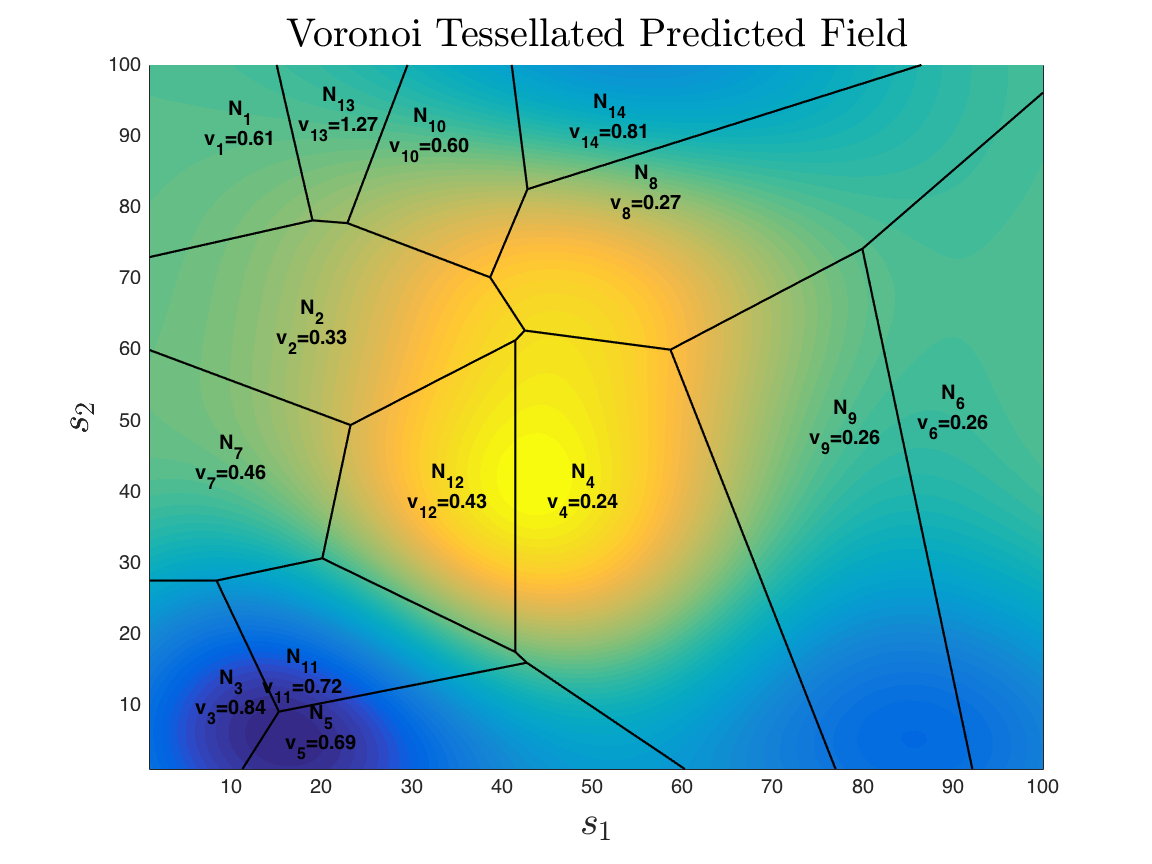
\includegraphics[width=0.8\textwidth]{./figures/natural_neighborhood_selection.png}
        \captionsetup{skip=0.0\baselineskip,size=footnotesize}
        \caption{Voronoi tessellations of the predicted field in Figure \ref{fig:krig_field}.}
        \label{fig:nat_neigh}
    \end{subfigure}
    \\
    \begin{subfigure}[b]{\textwidth}
        % \includegraphics[width=0.7\textwidth]{./figures/undir_graph_save.png}

        %https://tex.stackexchange.com/questions/270543/draw-a-graph-in-latex-with-tikz
        \centering
        \begin{tikzpicture}
        \begin{scope}[every node/.style={circle,thick,draw}]
            \node (N4) at (0.2,3) {$N_4$};
            \node (N2) at (1.6,.6) {$N_2$};
            \node (N7) at (4.5,.4) {$N_{7}$};
            \node (N12) at (2.7,3) {$N_{12}$};
            
        \end{scope}

        \begin{scope}[>={Stealth[black]},
                      every node/.style={fill=white,circle},
                      every edge/.style={draw=red,very thick}]

            \draw (N7) -- (4.6,1.8) [dashed];
            \draw (N7) -- (5.0,1.6) [dashed];

            \draw (N2) -- (0.4,1.5) [dashed];
            \draw (N2) -- (0.4,1.1) [dashed];
            \draw (N2) -- (0.0,0.9) [dashed];
            \draw (N2) -- (2.6,1.3) [dashed];

            \draw (N4) -- (1.0,2.6) [dashed];
            \draw (N4) -- (0.9,2.4) [dashed];
            \draw (N4) -- (0.4,1.8) [dashed];
            \draw (N4) -- (0,2.0) [dashed];

            \draw (N12) -- (3.9,2.7) [dashed];
            % edge[bend right=90] node
            \path [-] (N4) edge node {$w_{4,2}$} (N2);
            \path [-] (N4) edge node {$w_{4,12}$} (N12);
            \path [-] (N12) edge node {$w_{12,2}$} (N2);
            \path [-] (N12) edge node {$w_{12,7}$} (N7);
            \path [-] (N2) edge node {$w_{2,7}$} (N7);
            

        \end{scope}
        \end{tikzpicture}

        \captionsetup{skip=0.5\baselineskip,size=footnotesize}
        \caption{A subset of the weighted graph representing the adjacencies of the neighbors in Figure \ref{fig:nat_neigh}}
        \label{fig:neigh_graph}
  \end{subfigure}
  \captionsetup{skip=0.5\baselineskip,size=small}
  \caption{The predicted field is tessellated based on the measured point locations in \ref{fig:nat_neigh}. An undirected graph is constructed from the tessellations in \ref{fig:neigh_graph}. The label in each neighborhood identifies the neighborhood name, $\upsilon_i$, and the associated confidence of prediction, $\nu_i$, for that neighborhood.}
\end{figure}